\section{ESDIRK23}
Now another particular case of a Runge-Kutta method is the Explicit Singly Diagonal Implicit Runge-Kutta of 2nd order and 3rd order error estimation (ESDIRK23). The problem with Explicit Runge-Kutta methods is their relative small stability regions. None of them are A-stable and therefore neither L-stable. By spending the degrees of freedom cleverly as we will see, A-stability and L-stability can be achieved.

\\\

ESDIRK is family of methods sharing the same Butcher's Tableau, here illustrated for ESDIRK23 methods:

\begin{table}[H]
    \centering
\begin{tabular}{c|ccc}
0 & 0 & & \\
$c_{2}$ & $a_{21}$ & $\gamma$ & \\
1 & $b_{1}$ & $b_{2}$ & $\gamma$ \\
\hline$x_{n+1}$ & $b_{1}$ & $b_{2}$ & $\gamma$ \\
$\hat{x}_{n+1}$ & $\hat{b}_{1}$ & $\hat{b}_{2}$ & $\hat{b}_{3}$ \\
\hline$e_{n+1}$ & $d_{1}$ & $d_{2}$ & $d_{3}$
\end{tabular}
    \caption{Butcher's Tableau for the general ESDIRK23.}
    \label{tab:ESDIRK23general}
\end{table}

From $a_{1,1} = 0$ it follows that the method starts with an explicit step (saved from the previous iteration), i.e. $T_{1}=t_{n}, \quad X_{1}=x_{n}, \quad f_1 = f(t_n, x_n)$. Now the following two steps are implicit since the calculation of $X_2$ and $X_3$ \textit{depends} on $X_2$ and $X_3$ respectively. Note how they mutually share the same coefficient $\gamma$ making the method \textit{Singly Diagonal}. So how is $X_2$ and $X_3$ calculated implicitly? Using the Runge-Kutta equations \ref{eq:RKgeneral1} and \ref{eq:RKgeneral2} and using Newton's Method as explained in Section 3, we must solve

\begin{equation}
R\left(X_{2}\right)=X_{2}-h \gamma f\left(T_{2}, X_{2}\right)-x_{n}+h a_{21} f_{1}=0
\end{equation}
and
\begin{equation}
R\left(X_{3}\right)=X_{3}-h \gamma f\left(T_{3}, X_{3}\right)-x_{n}+h a_{31} f_{1}+h_{32} f_{2}=0
\end{equation}

Where $f_i = f(T_i, X_i)$. Note that since $c_3 = 1$, the 3rd stage corresponds to the full step $T_{3}=t_{n}+c_{3} h$ and therefore $x_{n+1} = X_3$. 



\subsection{Deriving ESDIRK23}
Now the question arises; What should the parameters be? By using the consistency condition 
\begin{equation}
C e=A e
\end{equation}

and order conditions (of order \textit{p)}

\begin{equation}
\Phi(\tau)=\frac{1}{\gamma(\tau)} \quad \forall r(\tau) \leq p
\end{equation}

and the table for the Taylor expansion terms \cite{JrgensenRunge-KuttaControl}:

\begin{equation}
\begin{array}{lcccccccc}
\hline \tau & \tau_{1} & \tau_{2} & \tau_{3} & \tau_{4} & \tau_{5} & \tau_{6} & \tau_{7} & \tau_{8} \\
r(\tau) & 1 & 2 & 3 & 3 & 4 & 4 & 4 & 4 \\
\sigma(\tau) & 1 & 1 & 2 & 1 & 6 & 1 & 2 & 1 \\
\gamma(\tau) & 1 & 2 & 3 & 6 & 4 & 8 & 12 & 24 \\
\Lambda(\tau) & I & C & C^{2} & A C & C^{3} & C A C & A C^{2} & A^{2} C \\
\Phi(\tau) & b^{\prime} e & b^{\prime} C e & b^{\prime} C^{2} e & b^{\prime} A C e & b^{\prime} C^{3} e & b^{\prime} C A C e & b^{\prime} A C^{2} e & b^{\prime} A^{2} C e \\
\Psi(\tau) & e & C e & C^{2} e & A C e & C^{3} e & C A C e & A C^{2} e & A^{2} C e \\
F(\tau) & f & f^{\prime} f & f^{\prime \prime}(f, f) & f^{\prime} f^{\prime} f & f^{\prime \prime \prime}(f, f, f) & f^{\prime \prime}\left(f, f^{\prime} f\right) & f^{\prime} f^{\prime \prime}(f, f) & f^{\prime} f^{\prime} f^{\prime} f \\
\hline
\end{array}
\caption{Functions on Rooted Trees.}
\end{equation}

We derive for the advancing method of order p=2:
\begin{align*}
    & b^T e = \frac{1}{1} \\
    & b^T C e = \frac{1}{2}
\end{align*}

And for the embedded method of order p=3:
\begin{align*}
    & \hat{b}^T e = \frac{1}{1} \\
    & \hat{b}^T C e = \frac{1}{2} \\
    & \hat{b}^T C^2 e = \frac{1}{3} \\
    & \hat{b}^T A C e = \frac{1}{6}
\end{align*}

Solving these equations there is still 1 degrees of freedom left. So choosing $\gamma=1-\frac{1}{\sqrt{2}}$ (see the attached Maple-sheet for details) we arrive at a well-defined ESDIRK23 which (by subtitution of coefficients) has the following Butcher's Tableau:

\begin{table}[H]
\centering
\begin{tabular}{c|ccc}
0 & 0 & 0 & 0 \\
$2-\sqrt{2}$ & $\frac{2-\sqrt{2}}{2}$  & $\frac{2-\sqrt{2}}{2}$ & 0 \\
$1$ & $\frac{\sqrt{2}}{4}$ & $\frac{\sqrt{2}}{4}$ & $\frac{2-\sqrt{2}}{2}$ \\ \hline
$x_{n+1}$ & $\frac{\sqrt{2}}{4}$ & $\frac{\sqrt{2}}{4}$ & $\frac{2-\sqrt{2}}{2}$ \\
$\hat{x}_{n+1}$ & $\frac{-\sqrt{2}+4}{12}$ & $\frac{3\sqrt{2}+4}{12}$ & $\frac{-\sqrt{2}+2}{6} $ \\ \hline
$e_{n+1}$ & $\frac{\sqrt{2}-1}{3}$ & $-\frac{1}{3}$ & $\frac{2-\sqrt{2}}{3}$
\end{tabular}
\caption{Butcher's Tableau of the derived ESDIRK23.}
\end{table}


Now as we shall see in the next section the choice of $\gamma$ was not a pure random one.

\subsection{Stability}
One can show as done in \cite{JrgensenRunge-KuttaControl} that the method is L-stable if and only if $\gamma = \frac{2-\sqrt{2}}{2} =1-\frac{1}{\sqrt{2}}$. The stability of the method can be seen in Figure \ref{fig:7_2}. Note that since $|R(z)| < 1$ for all $z$ where $\mathrm{Re}(z) < 0$ the method is A-stable. Additionally, $|R(z)|$ goes toward 0 as z approaches $-\infty$ and thus the method is L-stable. This is indicated by evaluating the transfer function in larger and larger negative numbers.

\begin{figure}[h]
    \centering
    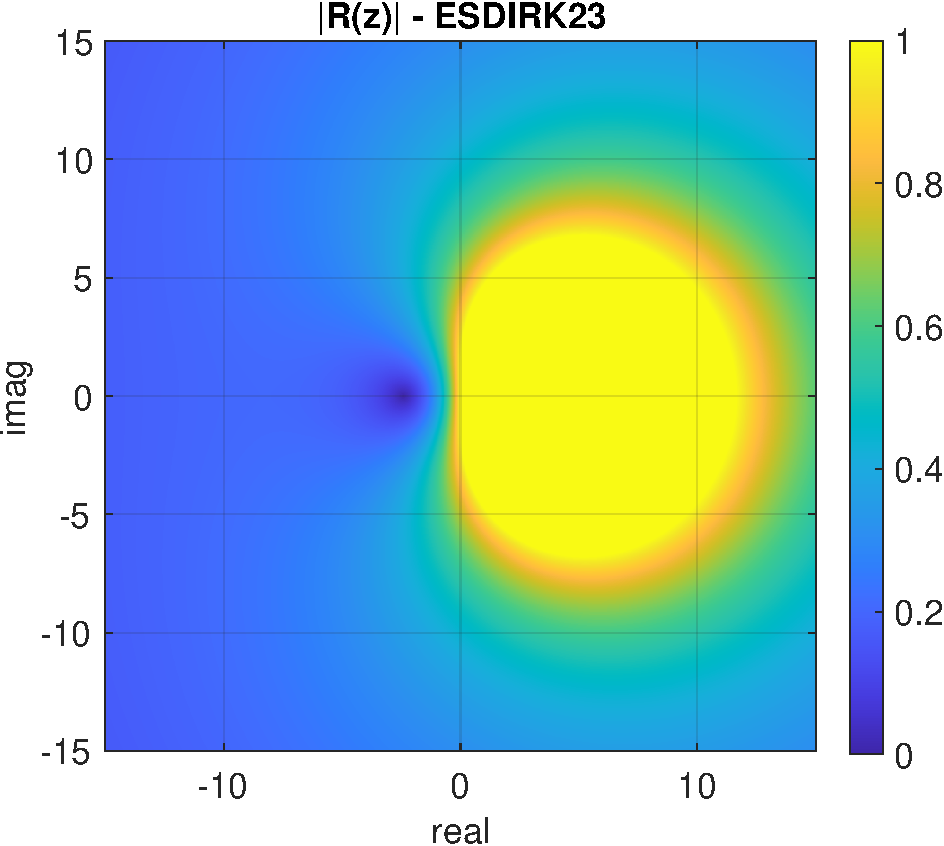
\includegraphics[width=0.7\textwidth]{plots/7_2a.pdf}
    \caption{Stability of derived ESDIRK23.}
    \label{fig:7_2}
\end{figure}

\subsection{MATLAB implementation}
The ESDIRK23 method with the Butcher's Tableau shown in Table 4 is implemented below. The implementation is largely based on the provided function.

\begin{adjustwidth*}{0cm}{-0.4cm}
\begin{lstlisting}[frame=single, language=Matlab,caption=ESDIRK23, label=ESDIRK23]
function [Tout,Xout,Gout,info,stats] = ESDIRK(fun,jac,t0,tf,x0,h0,...
    absTol,relTol,Method,varargin)
% Runge-Kutta method parameters
switch Method
    case 'myESDIRK23'
        gamma = 1-1/sqrt(2);
        a21 = 1 - sqrt(2)/2;
        b1 = sqrt(2)/4;
        b2 = b1;
        AT = [0 a21 b1;0 gamma b2;0 0 gamma];
        c  = [0; 2 - sqrt(2); 1];
        b  = AT(:,3);
        bhat = [   -sqrt(2)/12 + 1/3; ...
           sqrt(2)/4 + 1/3; ...
            -sqrt(2)/6 + 1/3    ];
        d  = b-bhat;
        p  = 2;
        phat = 3;
        s = 3;
end

% error and convergence controller
epsilon = 0.8;
tau = 0.1*epsilon; %0.005*epsilon;
itermax = 20;
ke0 = 1.0/phat;
ke1 = 1.0/phat;
ke2 = 1.0/phat;
alpharef = 0.3;
alphaJac = -0.2;
alphaLU  = -0.2;
hrmin = 0.01;
hrmax = 10;
%========================================================================
tspan = [t0 tf]; 
info = struct(...
            'Method',    Method,  ... 
            'nStage',    s,       ... 
            'absTol',    'dummy',  ... 
            'relTol',    'dummy',  ... 
            'iterMax',   itermax, ... 
            'tspan',     tspan,   ..
            'nFun',      0, ...
            'nJac',      0, ...
            'nLU',       0, ...
            'nBack',     0, ...
            'nStep',     0, ...
            'nAccept',   0, ...
            'nFail',     0, ...
            'nDiverge',  0, ...
            'nSlowConv', 0);


        
%% Main ESDIRK Integrator
%========================================================================
nx = size(x0,1);
F = zeros(nx,s);
t = t0;
x = x0;
h = h0;

[F(:,1),g]  = feval(fun,t,x,varargin{:});
info.nFun = info.nFun+1;
[dfdx,dgdx] = feval(jac,t,x,varargin{:});
info.nJac = info.nJac+1;
FreshJacobian = true;
if (t+h)>tf
    h = tf-t;
end
hgamma = h*gamma;
dRdx = dgdx - hgamma*dfdx;
[L,U,pivot] = lu(dRdx,'vector');
info.nLU = info.nLU+1;
hLU = h;

FirstStep = true;
ConvergenceRestriction = false;
PreviousReject = false;
iter = zeros(1,s);

% Output
chunk = 100;
Tout = zeros(chunk,1);
Xout = zeros(chunk,nx);
Gout = zeros(chunk,nx); 

Tout(1,1) = t;
Xout(1,:) = x.';
Gout(1,:) = g.';

while t<tf
    info.nStep = info.nStep+1;
    %=====================================================================
    % A step in the ESDIRK method
    i=1;   
    diverging = false;
    SlowConvergence = false;
    alpha = 0.0;
    Converged = true;
    while (i<s) && Converged
        % Stage i=2,...,s of the ESDIRK Method
        i=i+1;
        phi = g + F(:,1:i-1)*(h*AT(1:i-1,i));

        % Initial guess for the state
         if i==2
             dt = c(i)*h;
             G = g + dt*F(:,1);
             X = x + dgdx\(G-g);
         else
             dt = c(i)*h;
             G  = g + dt*F(:,1);
             X  = x + dgdx\(G-g);
         end
        T = t+dt;
            
        [F(:,i),G] = feval(fun,T,X,varargin{:});
        info.nFun = info.nFun+1;
        R = G - hgamma*F(:,i) - phi;
        rNewton = norm(R./(absTol + abs(G).*relTol),inf);
        Converged = (rNewton < tau);
        % Newton Iterations
        while ~Converged && ~diverging && ~SlowConvergence%iter(i)<itermax
            iter(i) = iter(i)+1;
            dX = U\(L\(R(pivot,1)));
            info.nBack = info.nBack+1;
            X = X - dX;
            rNewtonOld = rNewton;
            [F(:,i),G] = feval(fun,T,X,varargin{:});
            info.nFun = info.nFun+1;
            R = G - hgamma*F(:,i) - phi;
            rNewton = norm(R./(absTol + abs(G).*relTol),inf);
            alpha = max(alpha,rNewton/rNewtonOld);
            Converged = (rNewton < tau);
            diverging = (alpha >= 1);
            SlowConvergence = (iter(i) >= itermax); 
        end
        diverging = (alpha >= 1)*i;
    end
    %if diverging, i, iter, pause, end
    nstep = info.nStep;
    stats.t(nstep) = t;
    stats.h(nstep) = h;
    stats.r(nstep) = NaN;
    stats.iter(nstep,:) = iter;
    stats.Converged(nstep) = Converged;
    stats.Diverged(nstep)  = diverging;
    stats.AcceptStep(nstep) = false;
    stats.SlowConv(nstep)  = SlowConvergence*i;
    iter(:) = 0;
    %=====================================================================
    % Error and Convergence Controller
    if Converged
        % Error estimation
        e = F*(h*d);
        r = norm(e./(absTol + abs(G).*relTol),inf);
        CurrentStepAccept = (r<=1.0);
        r = max(r,eps);
        stats.r(nstep) = r;
        % Step Length Controller
        if CurrentStepAccept
            stats.AcceptStep(nstep) = true;
            info.nAccept = info.nAccept+1;
            if FirstStep || PreviousReject || ConvergenceRestriction
                % Aymptotic step length controller
                hr = 0.75*(epsilon/r)^ke0; 
            else
                % Predictive controller
                s0 = (h/hacc);
                s1 = max(hrmin,min(hrmax,(racc/r)^ke1));
                s2 = max(hrmin,min(hrmax,(epsilon/r)^ke2));
                hr = 0.95*s0*s1*s2;
            end
            racc = r;
            hacc = h;
            FirstStep = false;
            PreviousReject = false;
            ConvergenceRestriction = false;
            
            % Next Step
            t = T;
            x = X;
            g = G;
            F(:,1) = F(:,s);            
            
        else % Reject current step
            info.nFail = info.nFail+1;
            if PreviousReject
                kest = log(r/rrej)/(log(h/hrej));
                kest = min(max(0.1,kest),phat);
                hr   = max(hrmin,min(hrmax,((epsilon/r)^(1/kest))));
            else
                hr = max(hrmin,min(hrmax,((epsilon/r)^ke0)));
            end
            rrej = r;
            hrej = h;
            PreviousReject = true;
        end
   
        % Convergence control
        halpha = (alpharef/alpha);
        if (alpha > alpharef)
            ConvergenceRestriction = true;
            if hr < halpha
                h = max(hrmin,min(hrmax,hr))*h;
            else
                h = max(hrmin,min(hrmax,halpha))*h;
            end
        else
            h = max(hrmin,min(hrmax,hr))*h;
        end
        h = max(1e-8,h);
        if (t+h) > tf
            h = tf-t;
        end
        
        % Jacobian Update Strategy
        FreshJacobian = false;
        if alpha > alphaJac
            [dfdx,dgdx] = feval(jac,t,x,varargin{:});
            info.nJac = info.nJac+1;
            FreshJacobian = true;
            hgamma = h*gamma;
            dRdx = dgdx - hgamma*dfdx; 
            [L,U,pivot] = lu(dRdx,'vector');
            info.nLU = info.nLU+1;
            hLU = h;
        elseif (abs(h-hLU)/hLU) > alphaLU 
            hgamma = h*gamma;
            dRdx = dgdx-hgamma*dfdx;
            [L,U,pivot] = lu(dRdx,'vector');
            info.nLU = info.nLU+1;
            hLU = h;
        end        
    else % not converged
        info.nFail=info.nFail+1;
        CurrentStepAccept = false;
        ConvergenceRestriction = true;
        if FreshJacobian && diverging
            h = max(0.5*hrmin,alpharef/alpha)*h;
            info.nDiverge = info.nDiverge+1;
        elseif FreshJacobian
            if alpha > alpharef
                h = max(0.5*hrmin,alpharef/alpha)*h;
            else
                h = 0.5*h;
            end
        end
        if ~FreshJacobian
            [dfdx,dgdx] = feval(jac,t,x,varargin{:});
            info.nJac = info.nJac+1;
            FreshJacobian = true;
        end
        hgamma = h*gamma;
        dRdx = dgdx - hgamma*dfdx;
        [L,U,pivot] = lu(dRdx,'vector');
        info.nLU = info.nLU+1;
        hLU = h;
    end
    
    %=====================================================================
    % Storage of variables for output
    
    if CurrentStepAccept
       nAccept = info.nAccept;
       if nAccept > length(Tout);
           Tout = [Tout; zeros(chunk,1)];
           Xout = [Xout; zeros(chunk,nx)];
           Gout = [Gout; zeros(chunk,nx)];
       end
       Tout(nAccept,1) = t;
       Xout(nAccept,:) = x.';
       Gout(nAccept,:) = g.';
    end
end
info.nSlowConv = length(find(stats.SlowConv));
nAccept = info.nAccept;
Tout = Tout(1:nAccept,1);
Xout = Xout(1:nAccept,:);
Gout = Gout(1:nAccept,:);
\end{lstlisting}
\end{adjustwidth*}

\subsection{Van der Pol}
The solution from the above implementation on the Van der Pol problem can be seen in Figure \ref{fig:7_4}. ESDIRK23 solves the ODE with relative ease as seen by the few steps taken.

\begin{figure}[h]
    \centering
    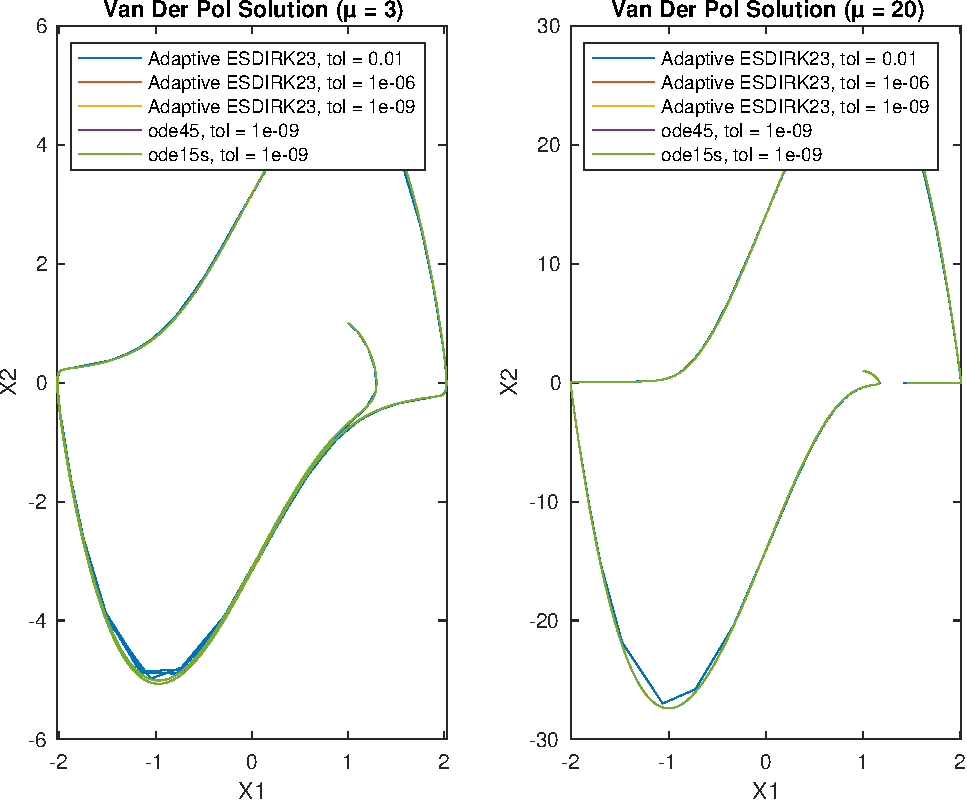
\includegraphics[width=\textwidth]{plots/7_4b.pdf}
    \caption{Solution of ESDIRK23 on the Van der Pol problem.}
    \label{fig:7_4}
\end{figure}

\subsection{Comparison with other solvers}



%\begin{table}[H]
%    \centering
%\begin{tabular}{c|ccc}
%0 & 0 & & \\
%$2 - \sqrt{2}$ & $1 - \frac{\sqrt{2}}{2}$ & $1 - \frac{\sqrt{2}}{2}$ & \\
%1 & $\frac{\sqrt{2}}{4}$ & $\frac{\sqrt{2}}{4}$ & $1 - \frac{\sqrt{2}}{2}$ \\
%\hline$x_{n+1}$ & $\frac{\sqrt{2}}{4}$ & $\frac{\sqrt{2}}{4}$ & $1 - \frac{\sqrt{2}}{2}$ \\
%$\hat{x}_{n+1}$ & $-\frac{\sqrt{2}}{12} + \frac{1}{3}$ & $\frac{\sqrt(2}{4}+\frac{1}{3}$ & %$-\frac{\sqrt{2}}{6} + \frac{1}{3}$ \\
%\hline$e_{n+1}$ & $\frac{\sqrt{2}}{3} - \frac{1}{3}$ & $-\frac{1}{3}$ & $\frac{2}{3} - \frac{\sqrt{2}}{3}$
%%   \caption{Caption}
 %   \label{tab:my_label}
%\end{table}
